\pdfminorversion=4
\documentclass[aspectratio=169]{beamer}

\mode<presentation>
{
  \usetheme{default}
  \usecolortheme{default}
  \usefonttheme{default}
  \setbeamertemplate{navigation symbols}{}
  \setbeamertemplate{caption}[numbered]
  \setbeamertemplate{footline}[frame number]  % or "page number"
  \setbeamercolor{frametitle}{fg=white}
  \setbeamercolor{footline}{fg=black}
} 

\usepackage[english]{babel}
\usepackage[utf8x]{inputenc}
\usepackage{tikz}
\usepackage{courier}
\usepackage{array}
\usepackage{bold-extra}
\usepackage{minted}
\usepackage[thicklines]{cancel}
\usepackage{fancyvrb}

\xdefinecolor{dianablue}{rgb}{0.18,0.24,0.31}
\xdefinecolor{darkblue}{rgb}{0.1,0.1,0.7}
\xdefinecolor{darkgreen}{rgb}{0,0.5,0}
\xdefinecolor{darkgrey}{rgb}{0.35,0.35,0.35}
\xdefinecolor{darkorange}{rgb}{0.8,0.5,0}
\xdefinecolor{darkred}{rgb}{0.7,0,0}
\definecolor{darkgreen}{rgb}{0,0.6,0}
\definecolor{mauve}{rgb}{0.58,0,0.82}

\title[2019-05-15-refinement-types-irishep]{Refinement types and other werid language features for physics}
\author{Jim Pivarski}
\institute{Princeton University -- IRIS-HEP}
\date{May 15, 2019}

\usetikzlibrary{shapes.callouts}

\begin{document}

\logo{\pgfputat{\pgfxy(0.11, 7.4)}{\pgfbox[right,base]{\tikz{\filldraw[fill=dianablue, draw=none] (0 cm, 0 cm) rectangle (50 cm, 1 cm);}\mbox{\hspace{-8 cm}
\includegraphics[height=1 cm]{princeton-logo-long.png}\hspace{0.1 cm}\raisebox{0.1 cm}{
\includegraphics[height=0.8 cm]{iris-hep-logo-long.png}}\hspace{0.1 cm}}}}}

\begin{frame}
  \titlepage
\end{frame}

\logo{\pgfputat{\pgfxy(0.11, 7.4)}{\pgfbox[right,base]{\tikz{\filldraw[fill=dianablue, draw=none] (0 cm, 0 cm) rectangle (50 cm, 1 cm);}\mbox{\hspace{-8 cm}
\includegraphics[height=1 cm]{princeton-logo.png}\hspace{0.1 cm}\raisebox{0.1 cm}{
\includegraphics[height=0.8 cm]{iris-hep-logo.png}}\hspace{0.1 cm}}}}}

% Uncomment these lines for an automatically generated outline.
%\begin{frame}{Outline}
%  \tableofcontents
%\end{frame}

% START START START START START START START START START START START START START

\begin{frame}{}
\large
\vspace{1.25 cm}
Quite a few groups have been thinking about physics event processing languages, explicitly or implicitly.

\vspace{0.25 cm}
\begin{itemize}
\item \textcolor{darkblue}{LHADA/ADL:} Sezen Sekmen, Harry Prosper, Philippe Gras
\item \textcolor{darkblue}{CutLang:} Gokhan Unel
\item \textcolor{darkblue}{IRIS-HEP Analysis Systems:} Gordon Watts, Mason Proffitt, Emma Torro
\item \textcolor{darkblue}{FAST-Carpenter (YAML):} Benjamin Krikler
\item \textcolor{darkblue}{NAIL:} Andrea Rizzi
\item \textcolor{darkblue}{RDataFrame:} Enrico Guiraud, Danilo Piparo, and the ROOT Team
\item \textcolor{darkblue}{AEACuS \& RHADAManTHUS:} Joel Walker (phenomenology)
\item \textcolor{darkblue}{Femtocode:} me, though not for several years\ldots
\end{itemize}

\vspace{0.25 cm}
\small \hfill See \textcolor{blue}{\href{https://indico.cern.ch/event/769263/timetable/}{Analysis Description Languages Workshop}} (last week).
\end{frame}

\begin{frame}{}
\Large
\vspace{1.25 cm}
\begin{center}
Originally, I was going to talk about refinement types \\ (a core feature of Femtocode), but this talk has grown.
\end{center}
\end{frame}

\begin{frame}{}
\vspace{1.25 cm}
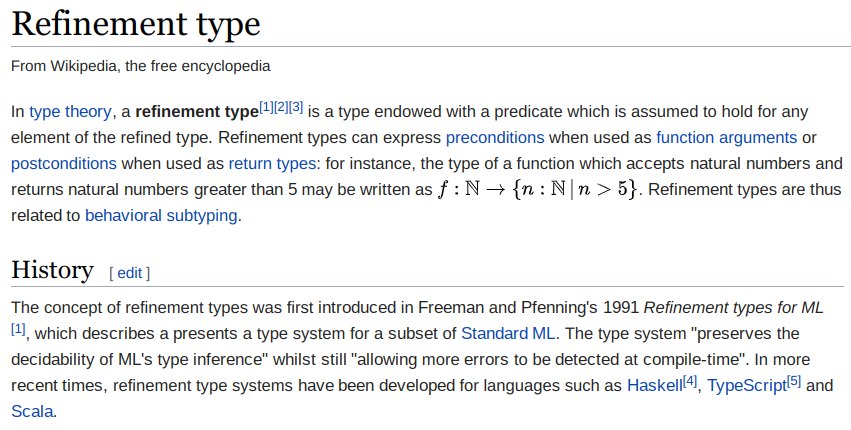
\includegraphics[width=\linewidth]{refinement-wikipedia.png}
\end{frame}

\begin{frame}[fragile]{Example in practice: \only<1-2>{prevent NaN at compile-time}\only<3-4>{identify impossible situations}}
\begin{columns}
\column{1.1\linewidth}
\begin{center}
\only<1>{\fbox{\mintinline{python}{x / y}}}\only<2>{\fbox{\mintinline{python}{if y != 0: x / y else: None}}}\only<3>{\fbox{\mintinline{python}{x == 5 and y == 6 and x == y}}}\only<4>{\fbox{\mintinline{python}{x == y and x == 5 and y == 6}}}
\end{center}

\begin{onlyenv}<1>
\begin{verbatim}
femtocode.parser.FemtocodeError: Function "/" does not accept
arguments with the given types:

    /(real,
      real)

    Indeterminate form (0 / 0) is possible; constrain with if-else.

Check line:col 1:0 (pos 0):

    x / y
----^
\end{verbatim}
\end{onlyenv}
\begin{onlyenv}<2>
\begin{verbatim}
----> union(null, real)











\end{verbatim}
\end{onlyenv}
\begin{onlyenv}<3>
\begin{verbatim}
femtocode.parser.FemtocodeError: Function "==" does not accept
arguments with the given types:

    ==(integer(min=5, max=5),
       integer(min=6, max=6))

    The argument types have no overlap (values can never be equal).

Check line:col 1:27 (pos 27):

    x == 5 and y == 6 and x == y
-------------------------------^
\end{verbatim}
\end{onlyenv}
\begin{onlyenv}<4>
\begin{verbatim}
femtocode.parser.FemtocodeError: Function "==" does not accept
arguments with the given types:

    ==(integer(min=5, max=5),
       integer(min=6, max=6))

    The argument types have no overlap (values can never be equal).

Check line:col 1:5 (pos 5):

    x == y and x == 5 and y == 6
---------^
\end{verbatim}
\end{onlyenv}
\end{columns}
\end{frame}

\begin{frame}{It's possible to turn {\it all} runtime errors into compile errors}
\large
\vspace{0.4 cm}
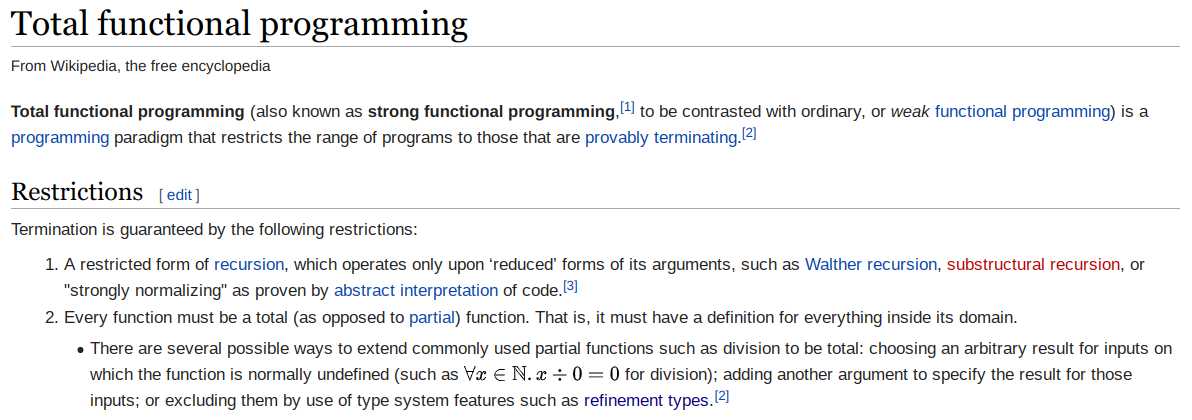
\includegraphics[width=0.98\linewidth]{totalfunctional-wikipedia.png}

\vspace{0.25 cm}
Including value sets in the type definitions lets us identify runtime conditions in the type-check.

\vspace{0.25 cm}
The hard parts are recursion (structural recursion) and infinite datasets (codata), both of which we can safely exclude from physics event processing.
\end{frame}

\begin{frame}[fragile]{Even without {\it total} functions, it can be useful for array lengths}
\large
\vspace{0.5 cm}

Awkward-Array users sometimes make this mistake:

\small\begin{minted}{python}
(nMuons > 0) & (Muons_pt[:, 0] > 30)    # intersection of masks
\end{minted}
\large

\vspace{0.25 cm}
The first mask requires events with at least one muon and the second requires the first muon to have 30~GeV, {\it but the selections are independent.}

\vspace{0.5 cm}
\begin{uncoverenv}<2->
The second fails because some events have no muons. The right way to do it is with a single selection:

\small\begin{minted}{python}
Muons_pt[(nMuons > 0), 0] > 30          # mask first dim, pick 0
\end{minted}
\end{uncoverenv}

\large

\vspace{0.25 cm}
\uncover<3->{\textcolor{darkblue}{The runtime error would be safer and more informative as a type error.}}
\end{frame}






\end{document}
